%%%%%%%%%%%%%%%%%%%%%%%%%%%%%%%%%%%%%%%%%
% Short Sectioned Assignment
% LaTeX Template
% Version 1.0 (5/5/12)
%
% This template has been downloaded from:
% http://www.LaTeXTemplates.com
%
% Original author:
% Frits Wenneker (http://www.howtotex.com)
%
% License:
% CC BY-NC-SA 3.0 (http://creativecommons.org/licenses/by-nc-sa/3.0/)
%
%%%%%%%%%%%%%%%%%%%%%%%%%%%%%%%%%%%%%%%%%

%----------------------------------------------------------------------------------------
%	PACKAGES AND OTHER DOCUMENT CONFIGURATIONS
%----------------------------------------------------------------------------------------

\documentclass[paper=a4, fontsize=12pt]{scrartcl} % A4 paper and 11pt font size

\usepackage[T1]{fontenc} % Use 8-bit encoding that has 256 glyphs
\usepackage{fourier} % Use the Adobe Utopia font for the document - comment this line to return to the LaTeX default
\usepackage[english]{babel} % English language/hyphenation
\usepackage{amsmath,amsfonts,amsthm} % Math packages

\usepackage{sectsty} % Allows customizing section commands
\allsectionsfont{\centering \normalfont\scshape} % Make all sections centered, the default font and small caps

\usepackage{graphicx}

\usepackage[a4paper,lmargin=2.5 cm,rmargin=2 cm,tmargin=2 cm,bmargin=2 cm]{geometry}

\usepackage{fancyhdr} % Custom headers and footers
\pagestyle{fancyplain} % Makes all pages in the document conform to the custom headers and footers
\fancyhead{} % No page header - if you want one, create it in the same way as the footers below
\fancyfoot[L]{} % Empty left footer
\fancyfoot[C]{} % Empty center footer
\fancyfoot[C]{\thepage} % Page numbering for right footer
\renewcommand{\headrulewidth}{0pt} % Remove header underlines
\renewcommand{\footrulewidth}{0pt} % Remove footer underlines
\setlength{\headheight}{13.6pt} % Customize the height of the header

\usepackage{chngcntr}
%\numberwithin{equation}{section} % Number equations within sections (i.e. 1.1, 1.2, 2.1, 2.2 instead of 1, 2, 3, 4)
%\numberwithin{figure}{section} % Number figures within sections (i.e. 1.1, 1.2, 2.1, 2.2 instead of 1, 2, 3, 4)
%\counterwithout{figure}{section}
%\numberwithin{table}{section} % Number tables within sections (i.e. 1.1, 1.2, 2.1, 2.2 instead of 1, 2, 3, 4)

\setlength\parindent{0pt} % Removes all indentation from paragraphs - comment this line for an assignment with lots of text

\usepackage{amsmath}
\usepackage{float} % To firce the location of figure
\usepackage{subfigure} %For side-by-side figures
\usepackage{lettrine}
%\usepackage{lipsum}
\usepackage{epstopdf} %To read *.eps Files
\usepackage{listings} % To include source codes in LATEX document
\usepackage{mathrsfs} % To include script fonts. use \mathscr{}
\usepackage{courier} % To write in courier fornt
\usepackage{mathtools} % For mat symbols
\usepackage{xfrac} % For \sfrac{}{}
%\usepackage{subcaption}
%----------------------------------------------------------------------------------------
%	TITLE SECTION
%----------------------------------------------------------------------------------------

\newcommand{\horrule}[1]{\rule{\linewidth}{#1}} % Create horizontal rule command with 1 argument of height

\title{	
\normalfont \normalsize 
\textsc{Wright State University\\ Department of Mechanical and Materials Engineering} \\ [25pt] % Your university, school and/or department name(s)
\horrule{0.5pt} \\[0.4cm] % Thin top horizontal rule
\large ME7690 - Vibration Testing and Machine Health Monitoring \\ % The assignment title
\huge Investigation Into Using Digital Filters For Post Processing of Response Data\\
\horrule{2pt} \\[0.4cm] % Thick bottom horizontal rule
}

\author{Admir Makas} % Your name

\date{\normalsize\today} % Today's date or a custom date

\begin{document}

\maketitle % Print the title

%----------------------------------------------------------------------------------------
%	PROBLEM 1
%----------------------------------------------------------------------------------------
\section*{Introduction}
Digital filters are extensively used in the electrical engineering community for varying purposes in order to obtain or isolate the particular signal of interest. In this report the discussion will be limited to low-pass and high-pass filters. In general, low-pass filters will pass all signals under some cutoff frequency. Conversely, high-pass filters will pass all signals over some cutoff frequency. In the present study, a high-pass filter constructed in Matlab was used in order to filter out undesirable noise in the response signals. During data gathering phase of a cantilever beam experiment, it was observed that the hammer and accelerometer signals possessed an offset and a very low frequency drift in the signal. This anomaly was detected after the fact and typically it should be addressed during the experimental set-up phase. Since data was already obtained, the decision was made to attempt a clean up of the data using a high-pass filter in order to remove the offset and drift before continuing with the data analysis.
\\
\\
Data used herein came from an experiment that aimed to study the effect of an unstable fixture on the beam response and subsequent cross spectrum density (CSD), transfer function (H1 and H2 estimation), and coherence calculations. Similar calculations were performed using the filtered data and compared to raw data calculations. Additionally, some pitfalls with using filters will be discussed in this report.
%
%
\section*{Filter Design}
As mentioned earlier Matlab was used to construct the high-pass filter used for cleaning up the data. Goal of the filter is to remove very low frequency content without affecting the actual beam response. The filer was invoked using function callout \textbf{[$fdesign.highpass$]}. The complete Matlab script can be seen in Figure~\ref{fig:FilterCode} below.
%
	\begin{figure}[H]
		\centering
		{
		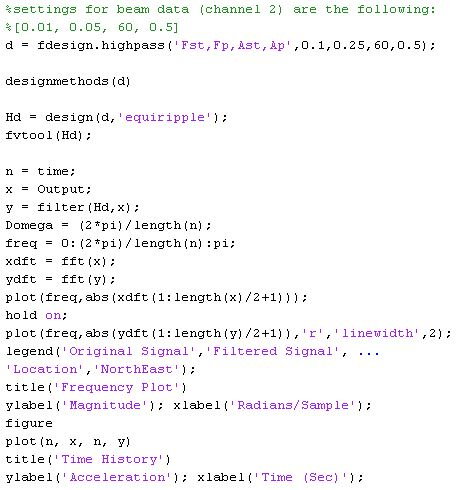
\includegraphics[height=16.0cm]{FilterCode.jpg}
		}
		\caption{High-pass filter code}
		\label{fig:FilterCode}
	\end{figure}
%
Besides the actual filter definition the code will also plot the raw and filtered signals for comparison. The plots are used to make judgments on the quality of the filtered signal. The filter uses four design parameters, which are defined in Table~\ref{table:filterParams}.
%
\begin{table}[H]
\centering
\begin{tabular}{ l | l }
		\textbf{Parameter} & \textbf{Definition} \\
	\hline                       
		Fst & Frequency at the beginning of the stop band. \\
	\hline
		Fp & Frequency at the end of the stop band. \\
	\hline
		Ast & Attenuation in the stop band window defined by Fst and Fp. \\
	\hline  
		Ap & Used to specify the allowable amount of ripple in the passed signal. \\
\end{tabular}
\caption{Filter paramaters}
\label{table:filterParams}
\end{table}
%
Appropriate values for the above parameters will filter the desired signal while maintaining the pertinent data. It should be noted that \textbf{Fst} and \textbf{Fp} must be given in terms of normalized frequency units, which ranges from 0 to 1. Remaining parameters \textbf{Ast}, and \textbf{Ap} are given in units of $dB$. Another useful graph supplied by the Matlab script is for the actual filter based on the input parameters. This enables the user to see changes made to the filter as parameters vary. Typical filter representation can be seen in Figure~\ref{fig:FilterDesign}.
%
	\begin{figure}[H]
		\centering
		{
		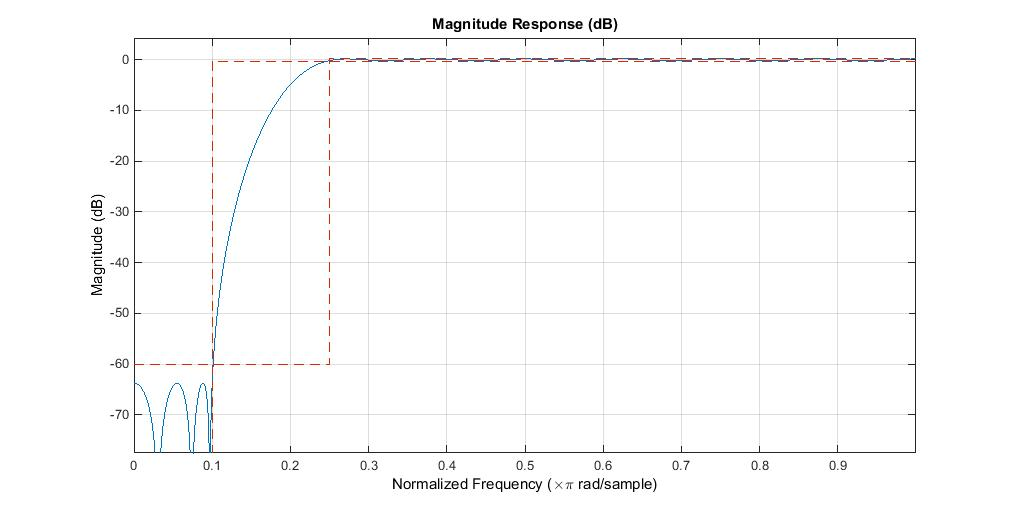
\includegraphics[height=8.0cm]{FilterDesign.jpg}
		}
		\caption{Graphical representation of the filter}
		\label{fig:FilterDesign}
	\end{figure}
%
The function of the aforementioned parameters is clearly visible in Figure~\ref{fig:FilterDesign}. In the graph the two vertical lines are defined by \textbf{Fst} and \textbf{Fp}, which define the stop band window. The floor of the frequency gain is \textbf{Ast}, which is the horizontal line passing through -60.0 dB. Finally, \textbf{Ap} is the small horizontal window specifying the allowable ripple, which is near the 0 dB line.
\\
\\
Filter parameters were modified until the desired filtered signal was obtained. Once the parameters were set, they were used to filter all the response signals of that type (e.g. beam response, or hammer input signal). This ensured that a family of signals were filtered with the same filter settings. This was done in order to remove any possibility of noise introduction due to changing filter parameters for each individual signal. Filtering of signals was performed on input and output signals with varying degree of success, which will be discussed in later sections.
\\
\\
A brief overview of the experimental set-up is provided for the cantilever beam, which generated the signals used in this report. Figure~\ref{fig:ExperimentSetup} shows the fixture configurations for FIXED and LOOSE setting. For the FIXED case, 50 lb weights were added to the corners of the fixture. Additionally, great care was taken to ensure ground was flat to prevent any high centering of the fixture.  In contrast, no weighted support was used for the LOOSE case and fixture was placed on the uneven section of the floor to facilitate worst case scenario.
%
	\begin{figure}[H]
		\centering
		\subfigure[Fixture set-up for FIXED condition]
		{
		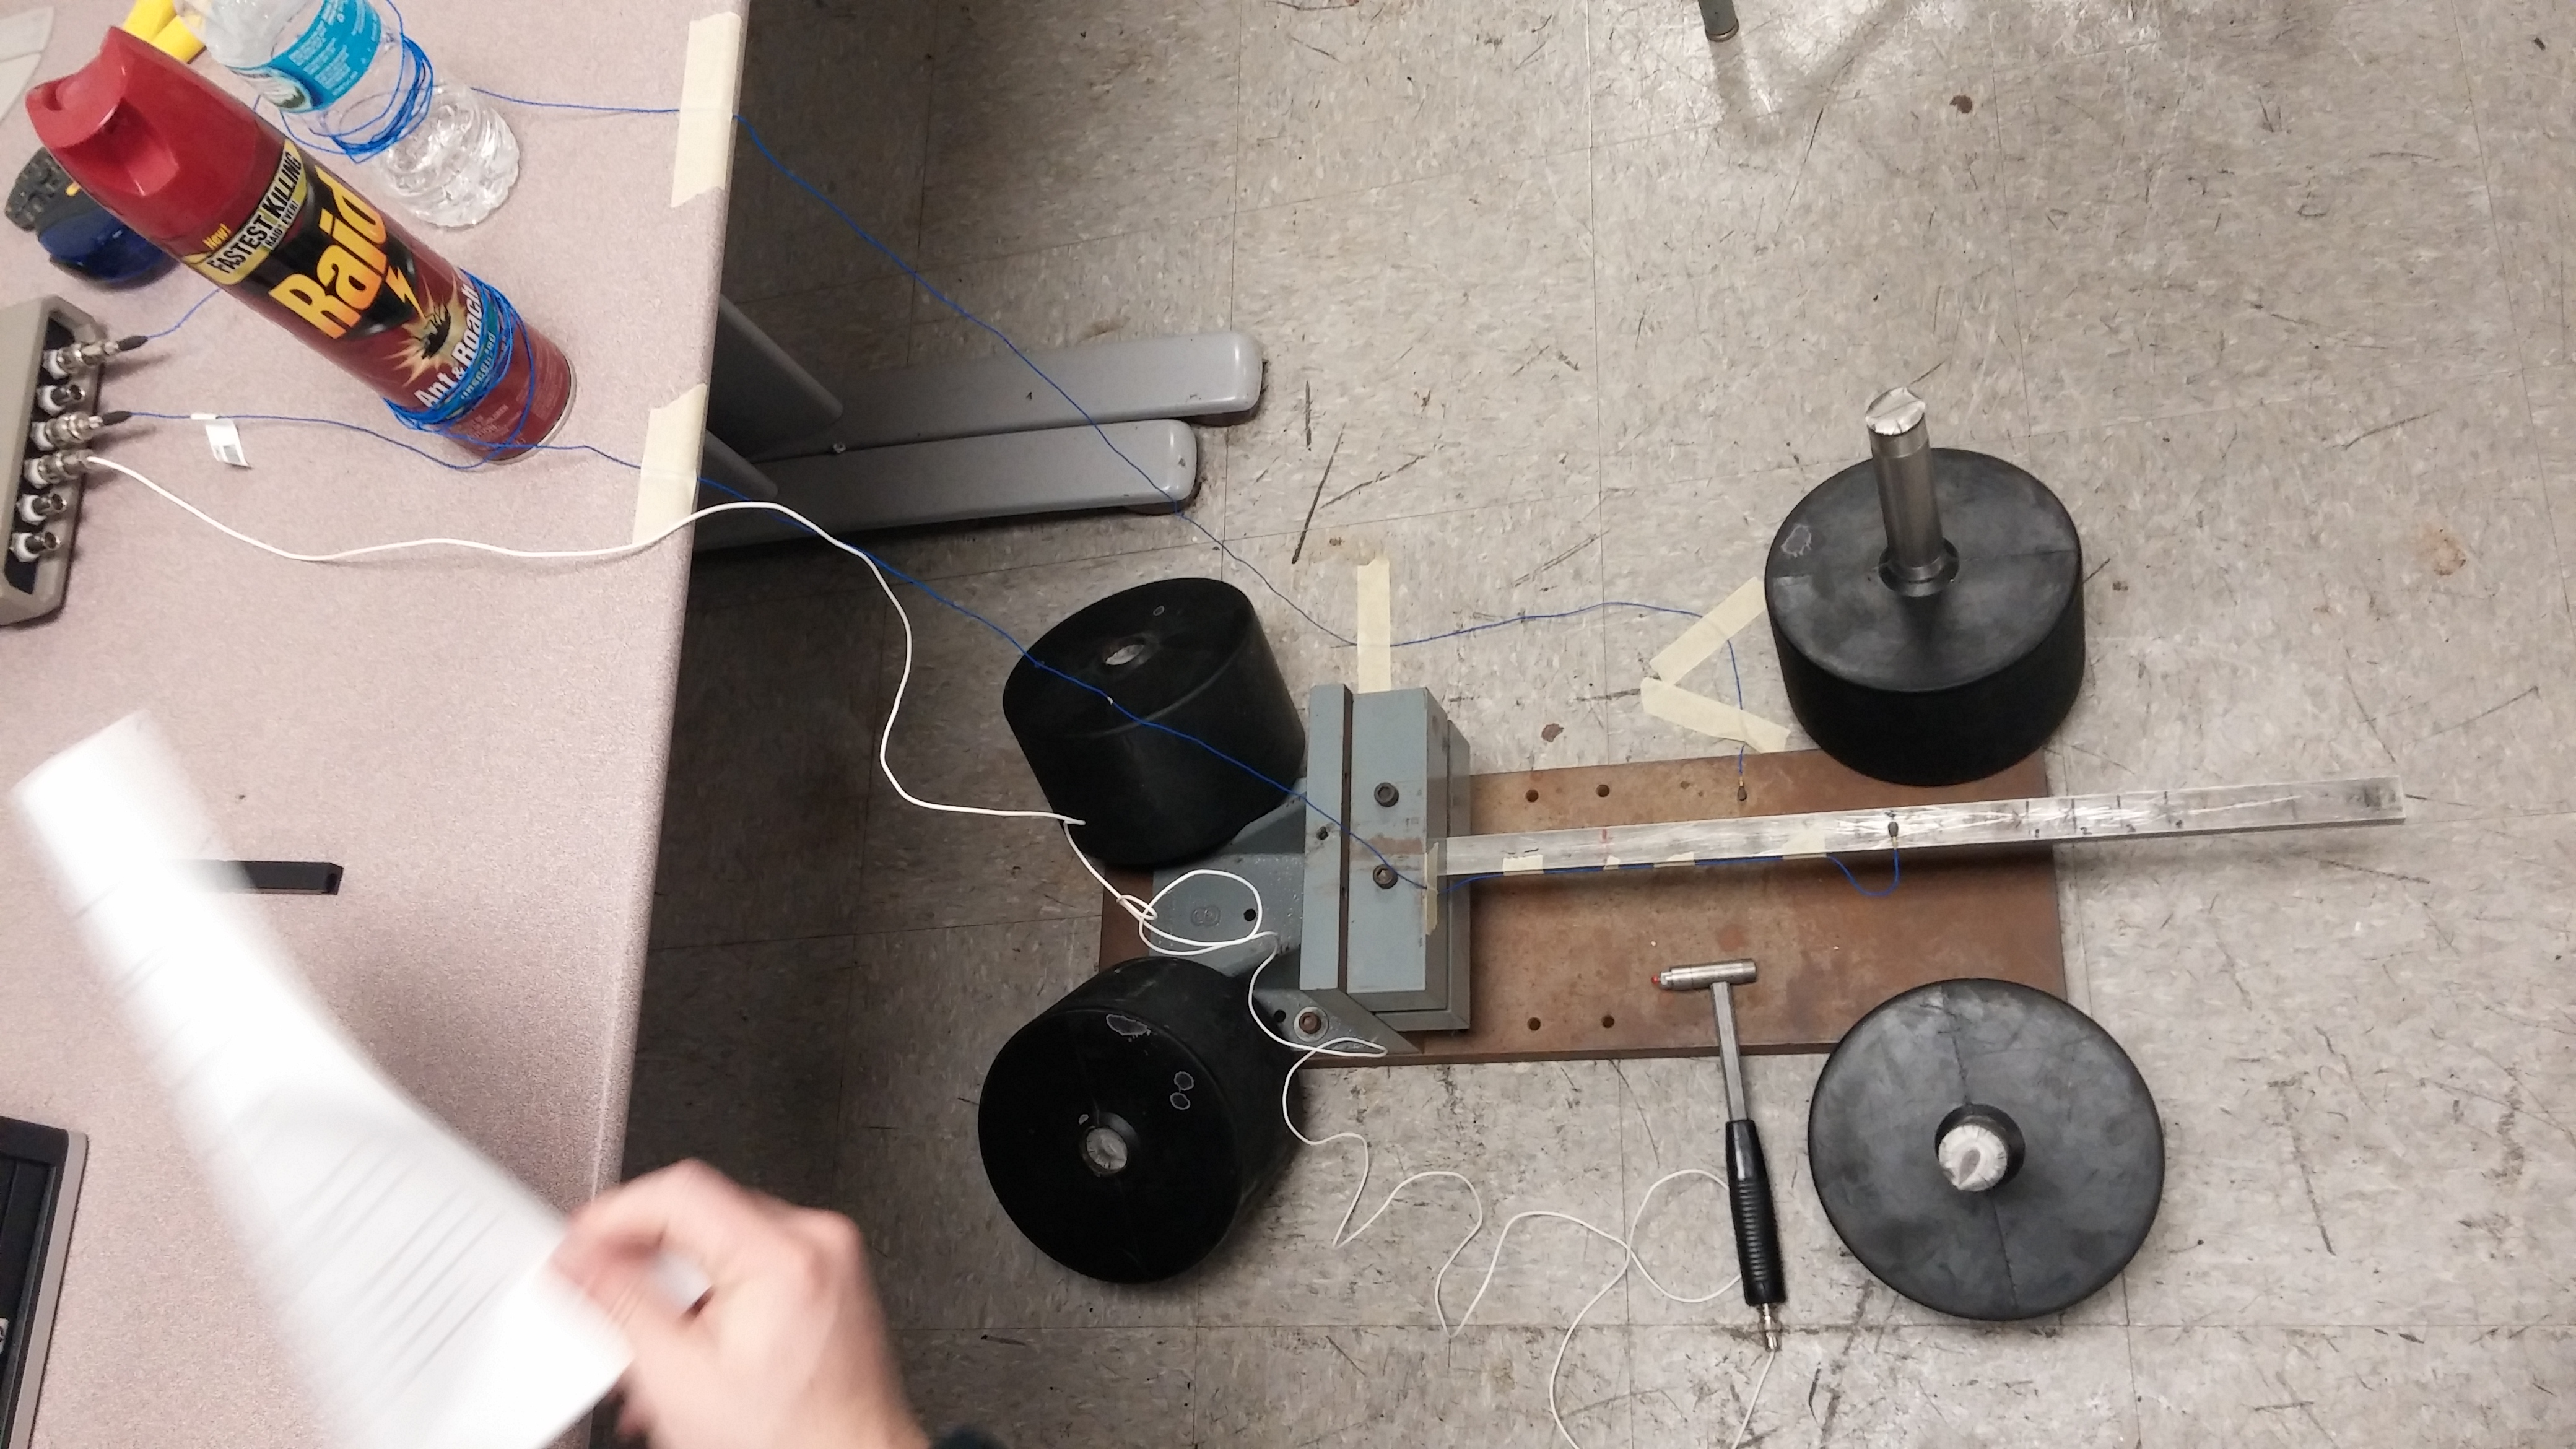
\includegraphics[height=5.0cm]{BeamWtWeight1.jpg}
		\label{fig:BeamWtWeight1}
		}
		\quad
		\subfigure[Fixture set-up for LOOSE condition]
		{
		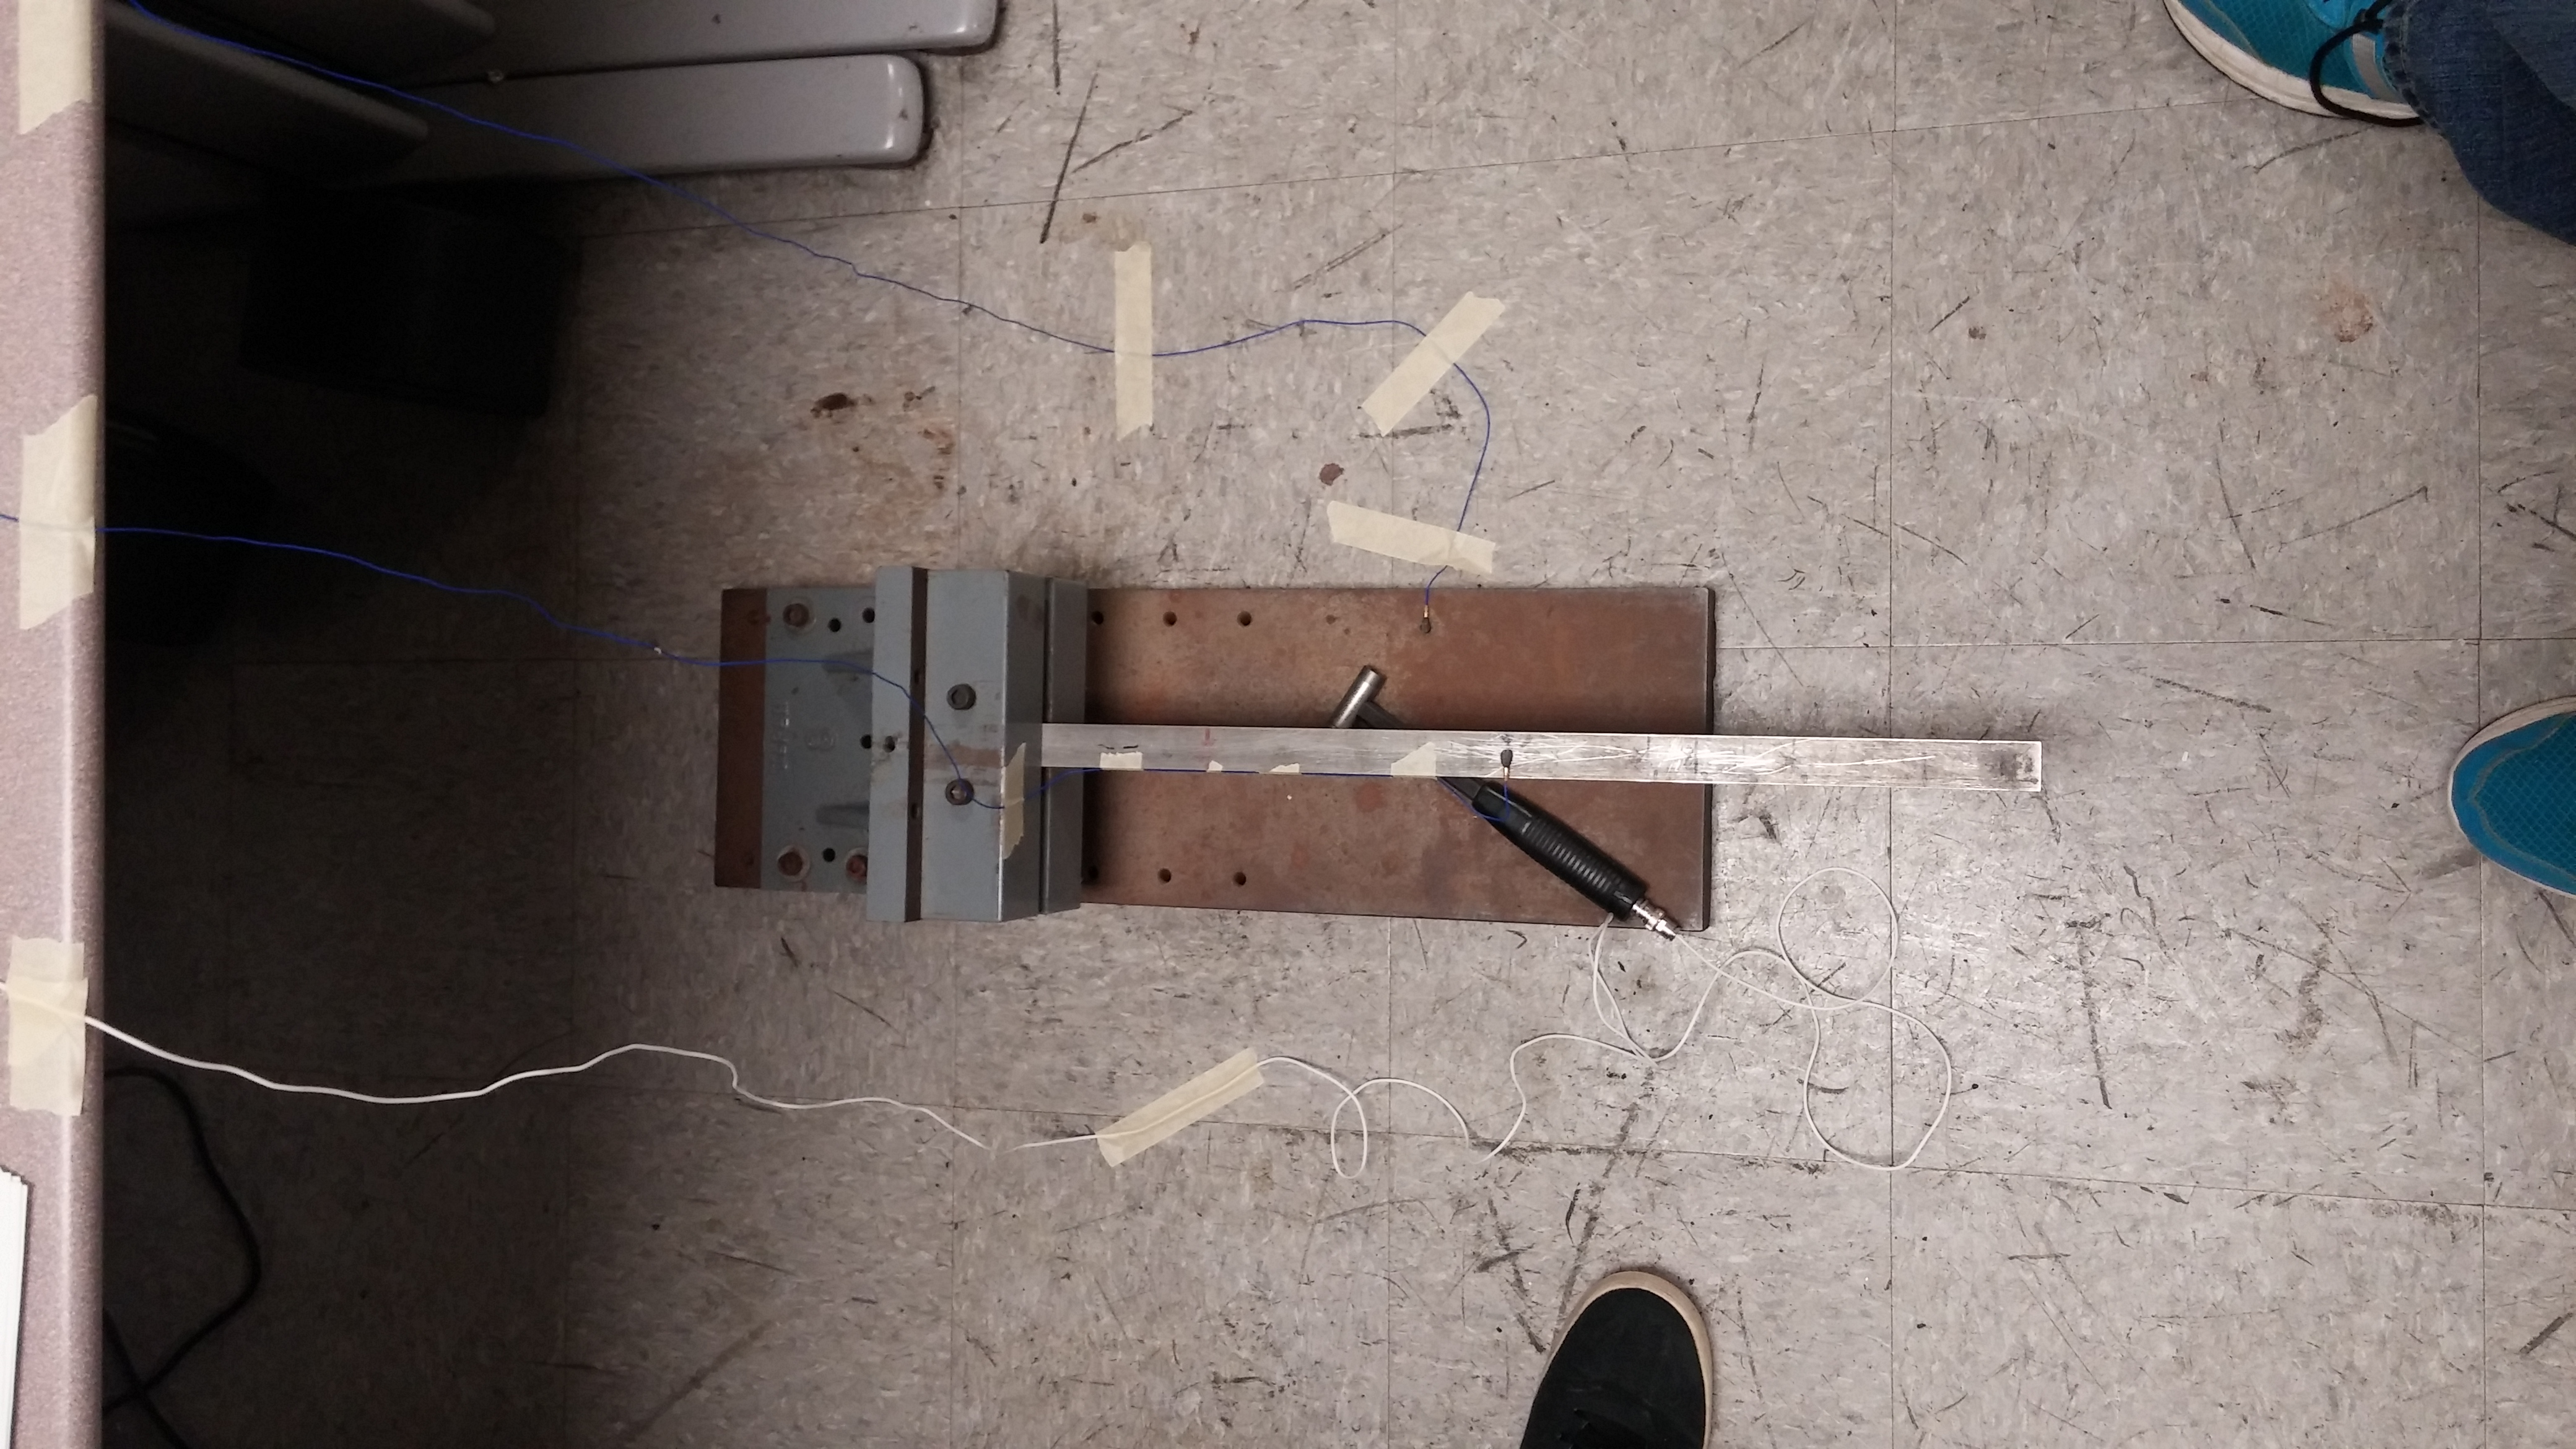
\includegraphics[height=5.0cm]{BeamNoWeight.jpg}
		\label{fig:BeamNoWeight}
		}
		\caption{Two experimental set-ups}
		\label{fig:ExperimentSetup}
	\end{figure}
%
A single accelerometer was placed on the beam and the fixture. Hammer excitation was carried out at two locations on the opposing ends of the beam. The excitation and measurement locations can be seen in Figure~\ref{fig:TopShot_mod}. Data sets generated by the two hammer strikes are dubbed 'base' and 'LOC4'. Additionally, two data samples were obtained when the hammer and accelerometers were in their respective boxes in order to account for random noise generated when the system was at rest.
%
	\begin{figure}[H]
		\centering
		{
		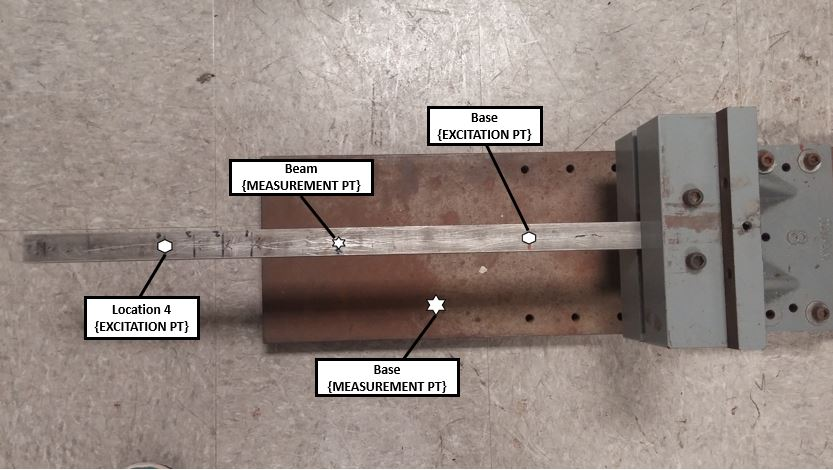
\includegraphics[height=7.0cm]{TopShot_mod.jpg}
		}
		\caption{Input and output locations of signal acquisition on the beam}
		\label{fig:TopShot_mod}
	\end{figure}
%
%
\section*{Data Filtering}
Attempts were made to filter both input and output signals generated for FIXED and LOOSE conditions. Filtering of the input signal was unsuccessful using the aforementioned filter design. Filtered signal had too many artificial artifacts that were not part of the original signal. As such it was deemed unusable for vibration analysis because the effect of the introduced artifacts was unknown. Figure~\ref{fig:inputSigFilter} shows the raw and filtered time signals and the zoomed region of interest.
%
	\begin{figure}[H]
		\centering
		\subfigure[Raw and filtered input signal]
		{
		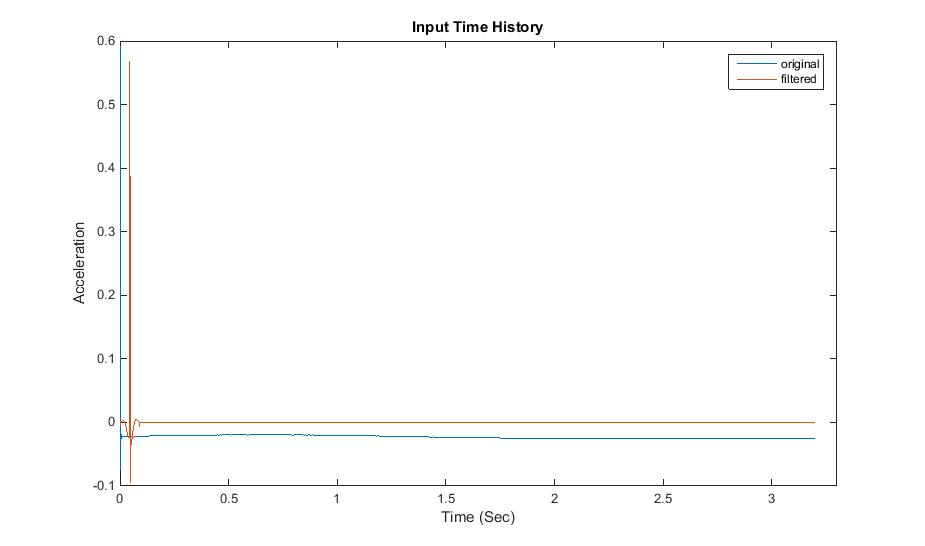
\includegraphics[height=5.50cm]{baseInputFilt_FIXED.jpg}
		\label{fig:baseInputFilt_FIXED}
		}
		\quad
		\subfigure[Raw and filtered input signal, closer look]
		{
		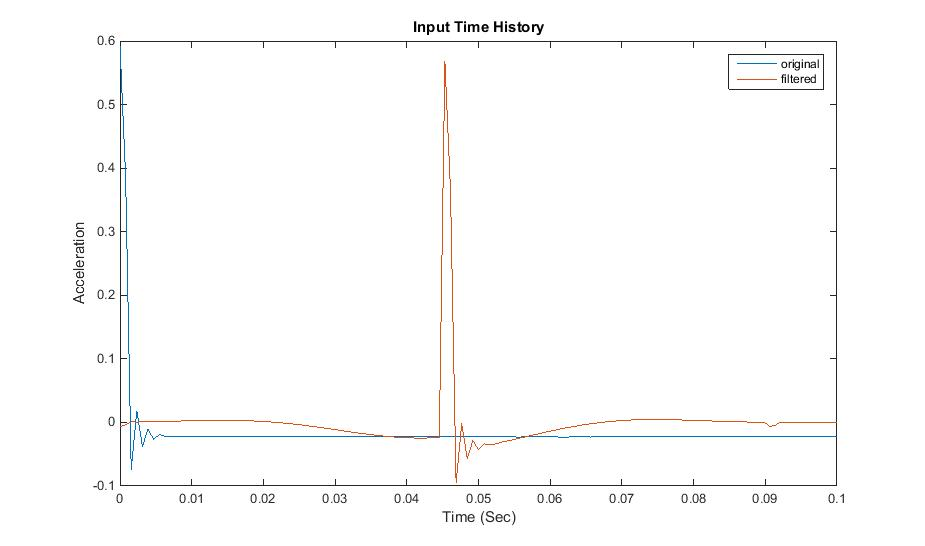
\includegraphics[height=5.50cm]{baseInputFiltZoom_FIXED.jpg}
		\label{fig:baseInputFiltZoom_FIXED}
		}
		\caption{Effect of filtering on input signal}
		\label{fig:inputSigFilter}
	\end{figure}
%
One obvious discrepancy is the horizontal translation of the signal. This is actually not a severe issue as this shift can be removed. The bigger problem is the change in the shape of the hammer spike. This was the case for all input signals. It is clear that there is low frequency content that cannot be removed from the hammer signal, which this type of filter will remove. Therefore, a different filtering scheme is needed for this type of signal. For the present case it was decided not perform any filtering on the signal. Rather, the vertical shift of the signal was treated using box data for the hammer.
\\
\\
Filtering the output beam data was more successful. The signal shift and drift were successfully removed without any apparent damage to the beam signal. Filtering was performed for both FIXED and LOOSE data sets with the same rate of success. As mentioned previously, same filter parameters were used for all the beam data filtered. Their respective values are listed in Table~\ref{table:filterVals}.
%
\begin{table}[H]
\centering
\begin{tabular}{ c | c }
		\textbf{Parameter} & \textbf{Value} \\
	\hline                       
		Fst & 0.01 \\
	\hline
		Fp & 0.05 \\
	\hline
		Ast & 60 \\
	\hline  
		Ap & 0.5 \\
\end{tabular}
\caption{Filter Values for beam data}
\label{table:filterVals}
\end{table}
%
For the base excitation, obtained filtered data agreed well with the raw data. The vertical shift and drift were successfully removed from the signal. As was the case with the hammer input signal there was a horizontal shift in the filtered data but it was manually removed from the signal. Figure~\ref{fig:outputSigFilterBase} shows a comparison between raw and filleted data.
%
	\begin{figure}[H]
		\centering
		\subfigure[Raw and filtered output signal, base]
		{
		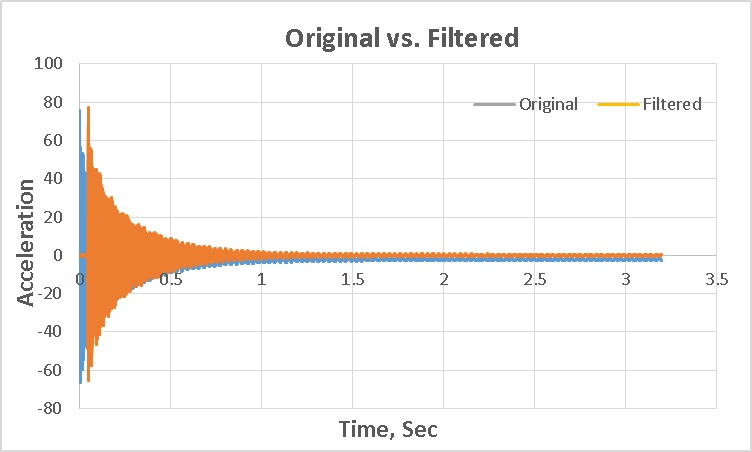
\includegraphics[height=5.50cm]{baseFiltvsOrig_Time_Plot_FIXED.jpg}
		\label{fig:baseFiltvsOrig_Time_Plot_FIXED}
		}
		\quad
		\subfigure[Raw and filtered output signal, base, closer look]
		{
		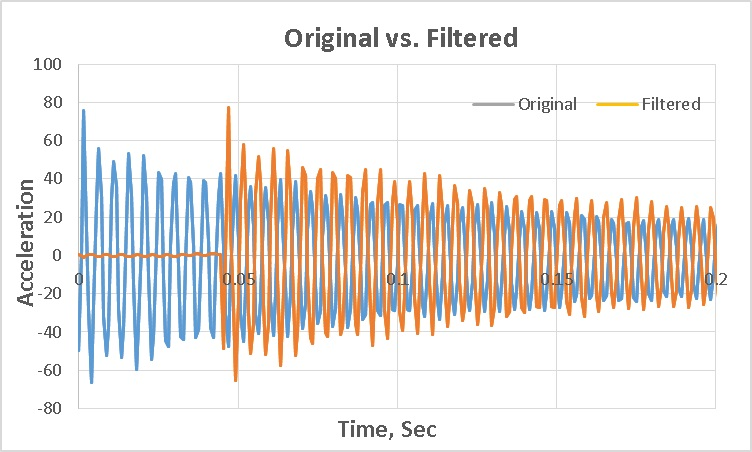
\includegraphics[height=5.50cm]{baseFiltvsOrig_Time_ZoomPlot_FIXED.jpg}
		\label{fig:baseFiltvsOrig_Time_ZoomPlot_FIXED}
		}
		\caption{Effect of filtering on output signal for base excitation}
		\label{fig:outputSigFilterBase}
	\end{figure}
%
The horizontal translation of the signal is clearly evident in Figure~\ref{fig:baseFiltvsOrig_Time_ZoomPlot_FIXED}. After manually removing the horizontal shift following time response is obtained in Figure~\ref{fig:ShiftoutputSigFilterBase}. Additionally, frequency plot is shown, which identifies the region that was filtered.
%
	\begin{figure}[H]
		\centering
		\subfigure[Raw compared to filtered output signal, translation removed, base]
		{
		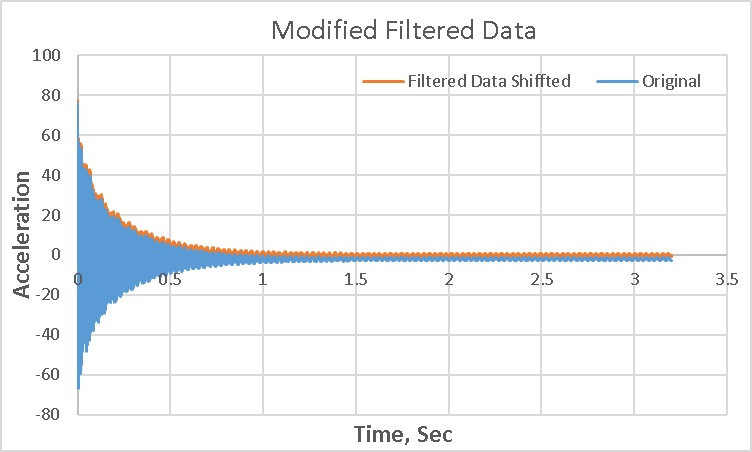
\includegraphics[height=5.50cm]{baseFiltShift_Time_Plot_FIXED.jpg}
		\label{fig:baseFiltShift_Time_Plot_FIXED}
		}
		\quad
		\subfigure[Frequency plot of raw and shifted beam signal, base]
		{
		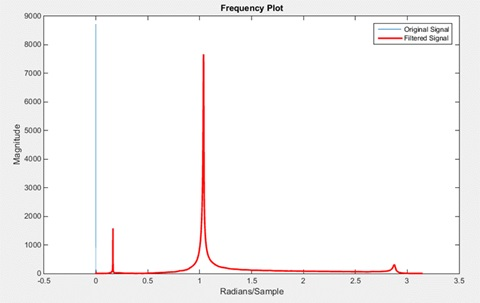
\includegraphics[height=5.50cm]{basewtWeight_freqPlot_FIXED.jpg}
		\label{fig:basewtWeight_freqPlot_FIXED}
		}
		\caption{Filtered signal with horizontal translation removed, base}
		\label{fig:ShiftoutputSigFilterBase}
	\end{figure}
%
Filtered time signal maintains the beam response while removing the vertical shift and drift, which were imparted by the accelerometer. Figure~\ref{fig:basewtWeight_freqPlot_FIXED} shows the frequency range that was removed from the shifted signal on the far left. The frequency plot clearly illustrates that the peaks of the filtered data match exactly with the original signal. Therefore, implying the beam response signal was not damaged by the filtering process.
\\
\\
Same process was performed on the beam data when hammer was used on LOC4. The filtered signal quality is the same as that of the base excitation data. Following Figures illustrate the filtering process.
%
	\begin{figure}[H]
		\centering
		\subfigure[Raw and filtered output signal, LOC4]
		{
		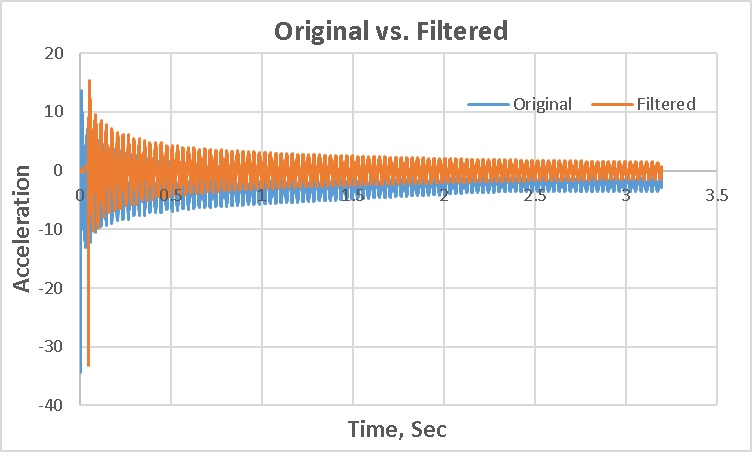
\includegraphics[height=5.50cm]{LOC4FiltvsOrig_Time_Plot_FIXED.jpg}
		\label{fig:LOC4FiltvsOrig_Time_Plot_FIXED}
		}
		\quad
		\subfigure[Raw and filtered output signal, LOC4, closer look]
		{
		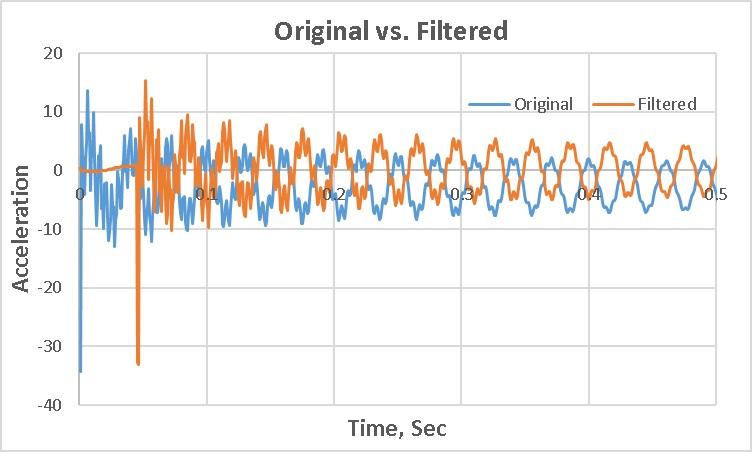
\includegraphics[height=5.50cm]{LOC4FiltvsOrig_Time_ZoomPlot_FIXED.jpg}
		\label{fig:LOC4FiltvsOrig_Time_ZoomPlot_FIXED}
		}
		\caption{Effect of filtering on output signal for LOC4 excitation}
		\label{fig:outputSigFilterLOC4}
	\end{figure}
%
Similar type of horizontal shift in the data is observed in Figure~\ref{fig:LOC4FiltvsOrig_Time_ZoomPlot_FIXED}. The shift was removed manually following same process used on the base data. The shifted and filtered signal along with the frequency plot are shown in Figure~\ref{fig:ShiftoutputSigFilterLOC4}. Again the removed frequency content is on the far left side of the Figure~\ref{fig:LOC4wtWeight_freqPlot_FIXED}. Beam response peaks are unaffected by the filtering process. A closer look at Figure~\ref{fig:LOC4wtWeight_freqPlot_FIXED} shows a very small amplitude at the second pole, which is roughly at 200 Hz. This will become important for the LOOSE fixture case since added noise will act to mask this pole.
%
	\begin{figure}[H]
		\centering
		\subfigure[Raw compared to filtered output signal, translation removed, LOC4]
		{
		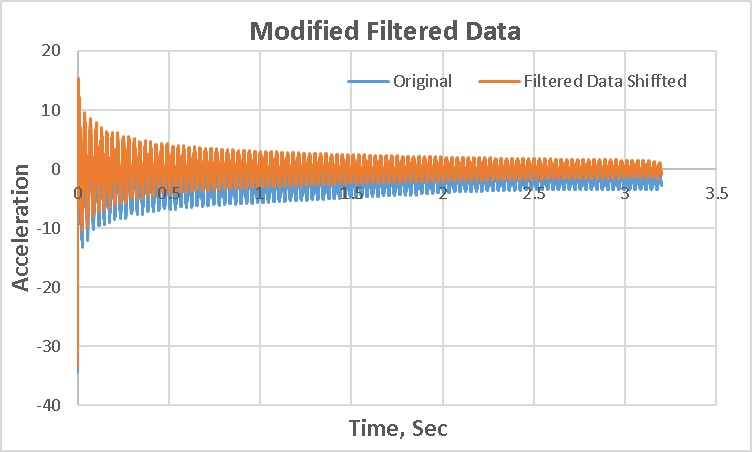
\includegraphics[height=5.50cm]{LOC4FiltShift_Time_Plot_FIXED.jpg}
		\label{fig:LOC4FiltShift_Time_Plot_FIXED}
		}
		\quad
		\subfigure[Frequency plot of raw and shifted beam signal, LOC4]
		{
		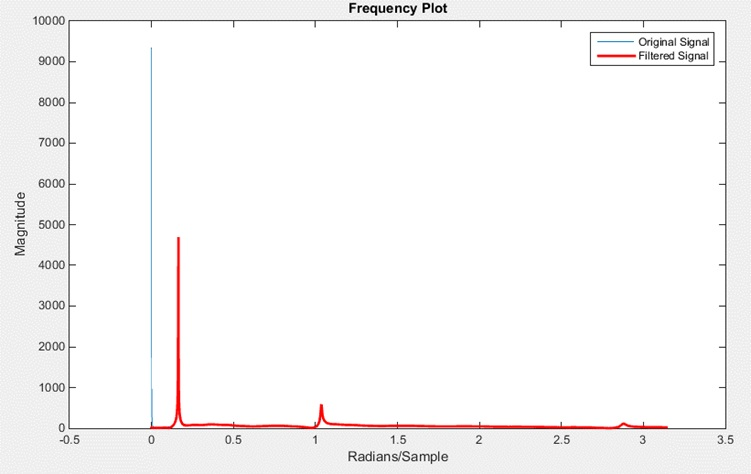
\includegraphics[height=5.50cm]{LOC4wtWeight_freqPlot_FIXED.jpg}
		\label{fig:LOC4wtWeight_freqPlot_FIXED}
		}
		\caption{Filtered signal with horizontal translation removed, LOC4}
		\label{fig:ShiftoutputSigFilterLOC4}
	\end{figure}
%
Next, a brief discussion is presented on pitfalls of data filtering due to improper filter parameter selection. Figure~\ref{fig:badFiltering} shows the case where the filter is removing the beam response. Time history in Figure~\ref{fig:badTimePlot} shows the removal of the first frequency from the response due to over-filtering. This effect is easier to identify in the frequency plot in Figure~\ref{fig:badFreqPlot} where the first peak is completely removed. Additionally, the second peak amplitude is reduced by a small margin. This simple case illustrates the importance of evaluating the time and frequency plots to ensure over-filtering is not taking place.
%
	\begin{figure}[H]
		\centering
		\subfigure[Effect of excessive filtering on time signal]
		{
		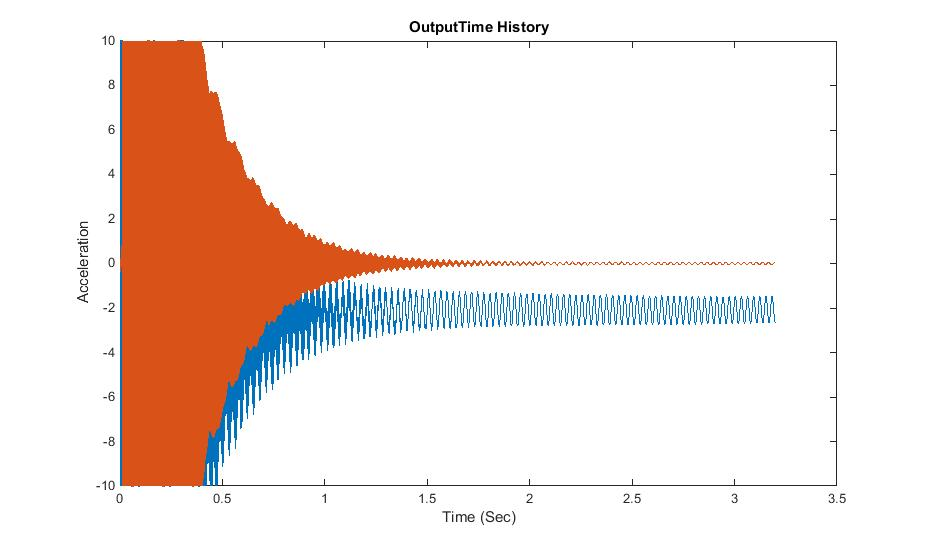
\includegraphics[height=6.50cm]{badTimePlot.jpg}
		\label{fig:badTimePlot}
		}
		\quad
		\subfigure[Effect of excessive filtering on frequency response]
		{
		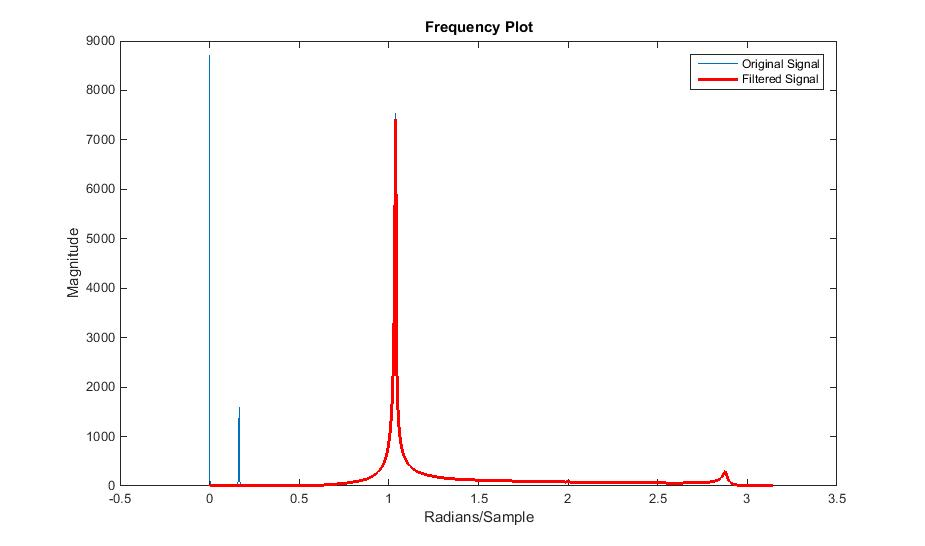
\includegraphics[height=6.50cm]{badFreqPlot.jpg}
		\label{fig:badFreqPlot}
		}
		\caption{Induced errors due to excessive filtering}
		\label{fig:badFiltering}
	\end{figure}
%
In summary, an attempt was made to filter the input and output signals. Filtering of the input data using the defined filter did not yield acceptable results. Therefore, the decision was made to use raw input signals and adjust them with the response of the hammer while in the box. Filtering of the output beam data yielded very agreeable results. The vertical shift and drift due to the sensor bias were successfully removed from the data while maintaining the beam response signal intact. Filtering was performed on all beam response data using filter parameters defined in Table~\ref{table:filterVals}.
%
%
\section*{Data Analysis}
Filtered data was used in conjunction with the vibration toolbox to generate results for the CSD, FRF, and coherence plots. These were compared with similar plots created using the raw data. Both FIXED and LOOSE data sets are compared. Starting with the FIXED data Figure~\ref{fig:baseFilt_wtWeight_CSD} thru~\ref{fig:baseR_woWeight_CSD} show CSD results.
%
	\begin{figure}[H]
		\centering
		\subfigure[CSD for base excitation using filtered data (FIXED)]
		{
		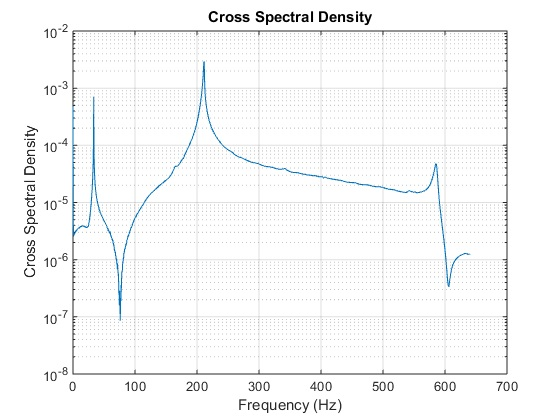
\includegraphics[height=5.50cm]{baseFilt_wtWeight_CSD.jpg}
		\label{fig:baseFilt_wtWeight_CSD}
		}
		\quad
		\subfigure[CSD for base excitation using filtered data (LOOSE)]
		{
		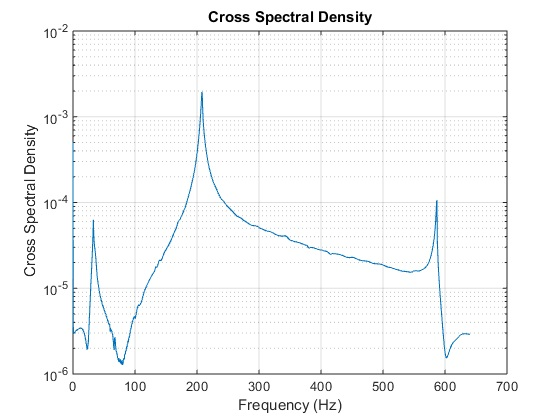
\includegraphics[height=5.50cm]{baseFilt_woWeight_CSD.jpg}
		\label{fig:baseFilt_woWeight_CSD}
		}
		%\quad
		\subfigure[CSD for base excitation using raw data (FIXED)]
		{
		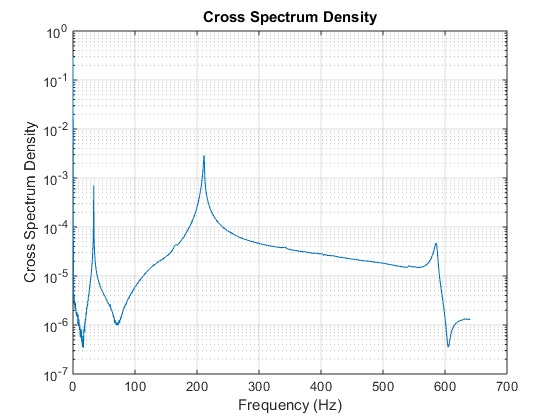
\includegraphics[height=5.50cm]{baseR_wtWeight_CSD.jpg}
		\label{fig:baseR_wtWeight_CSD}
		}
		%\quad
		\subfigure[CSD for base excitation using raw data(LOOSE)]
		{
		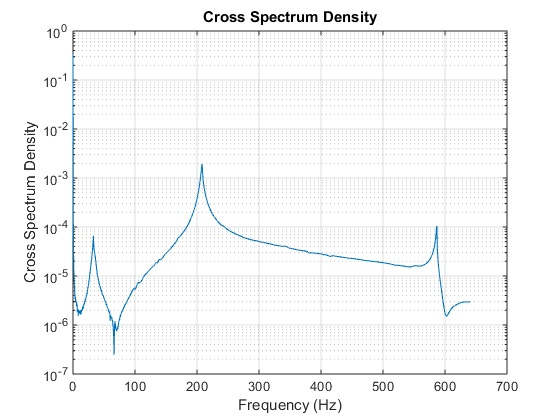
\includegraphics[height=5.50cm]{baseR_woWeight_CSD.jpg}
		\label{fig:baseR_woWeight_CSD}
		}
		\caption{CSD plots for base excitation. Results shown for FIXED and LOOSE condition.}
		\label{fig:FiltBaseCSDFigs}
	\end{figure}
%
First thing to note in Figure~\ref{fig:FiltBaseCSDFigs} is the fact that the amplitudes of the poles has not been affected by the filtering procedure, which is the desired result. Overall the shape of the CSD plots remains the same for raw and filtered results except for few locations. Largest impact of filtering is at the low frequency (0-50 Hz) portion of the plots. This is to be expected since the goal of the filtering procedure was to remove low frequency content and vertical shift imposed by the sensor noise. Zeroes of the filtered data are more pronounced due to noise removal. This is evident for FIXED and LOOSE settings. For the LOOSE data in Figure~\ref{fig:baseFilt_woWeight_CSD}, the location of the zero was shifted slightly to the right and begins to take on the shape of the raw FIXED CSD plot in Figure~\ref{fig:baseR_wtWeight_CSD}.
\\
\\
Next set of plots show the H1 and H2 estimations for the raw and filtered data. Comparing Figures~\ref{fig:baseFilt_wtWeight_H1_H2} and~\ref{fig:baseR_wtWeight_H1_H2_2} there is an interesting artifact that become pronounced for the H2 estimation of the filtered data at the frequency of 75 Hz. At this time it is not known why this occurred. Upon closer inspection of Figure~\ref{fig:baseR_wtWeight_H1_H2_2} the artifact is slightly showing, which indicates this feature was not altogether generated by the filtering process. It is, however, exacerbated by applying the filter. This discrepancy is clearly visible in the phase diagrams of Figures~\ref{fig:baseFilt_wtWeight_H1_H2} and~\ref{fig:baseR_wtWeight_H1_H2_2} where no zero is registered for the filtered data. Rather, the artificial peak implies a pole at this locations and as a result there is a negative phase shift at this location for Figure~\ref{fig:baseFilt_wtWeight_H1_H2}.
%
	\begin{figure}[H]
		\centering
		\subfigure[H1 and H2 for base excitation using filtered data (FIXED)]
		{
		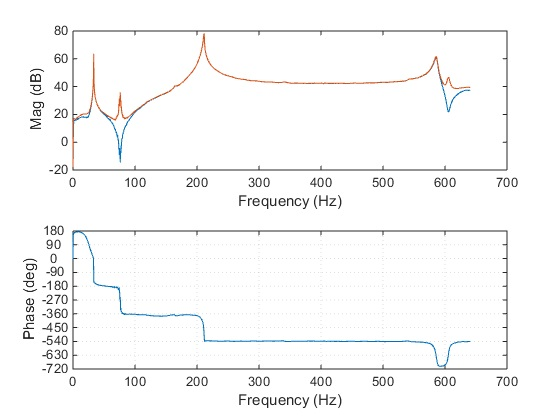
\includegraphics[height=5.50cm]{baseFilt_wtWeight_H1_H2.jpg}
		\label{fig:baseFilt_wtWeight_H1_H2}
		}
		\quad
		\subfigure[H1 and H2 for base excitation using filtered data (LOOSE)]
		{
		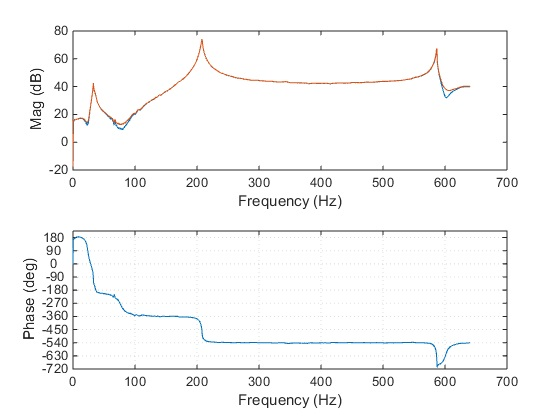
\includegraphics[height=5.50cm]{baseFilt_woWeight_H1_H2.jpg}
		\label{fig:baseFilt_woWeight_H1_H2}
		}
		%\quad
		\subfigure[H1 and H2 for base excitation using raw data (FIXED)]
		{
		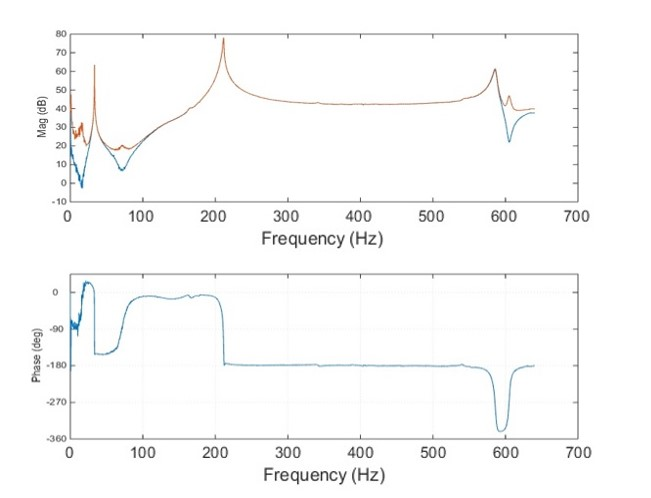
\includegraphics[height=5.50cm]{baseR_wtWeight_H1_H2_2.jpg}
		\label{fig:baseR_wtWeight_H1_H2_2}
		}
		%\quad
		\subfigure[H1 and H2 for base excitation using raw data(LOOSE)]
		{
		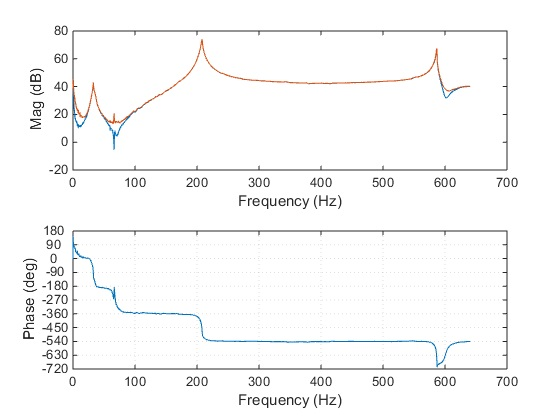
\includegraphics[height=5.50cm]{baseR_woWeight_H1_H2.jpg}
		\label{fig:baseR_woWeight_H1_H2}
		}
		\caption{H1 and H2 plots for base excitation. Results shown for FIXED and LOOSE condition.}
		\label{fig:FiltBaseH1H2Figs}
	\end{figure}
%
Removal of noise at the low frequencies does improve the initial plot shapes for both the FRF estimations and phase diagrams. For the LOOSE plots in Figures~\ref{fig:baseFilt_woWeight_H1_H2} and~\ref{fig:baseR_woWeight_H1_H2} there is a clear improvement in noise reduction for the filtered data. However, the phase diagram of the filtered data does not show the expected zero at the 75 Hz location. In fact the phase plots look very similar except the fact that the filtered data plots look smoother due to noise removal.
\\
\\
Final set of plots show the coherence calculations for raw and filtered data sets.
%
	\begin{figure}[H]
		\centering
		\subfigure[Coherence for base excitation using filtered data (FIXED)]
		{
		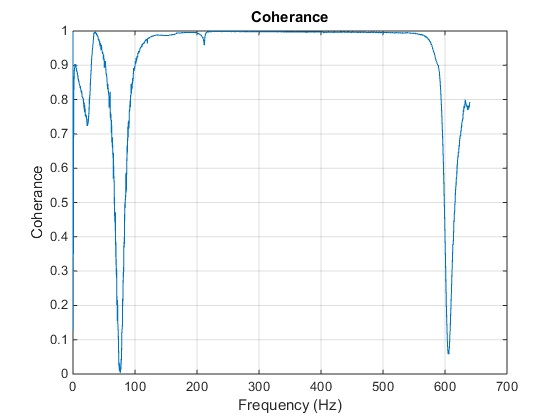
\includegraphics[height=5.50cm]{baseFilt_wtWeight_coh.jpg}
		\label{fig:baseFilt_wtWeight_coh}
		}
		\quad
		\subfigure[Coherence for base excitation using filtered data (LOOSE)]
		{
		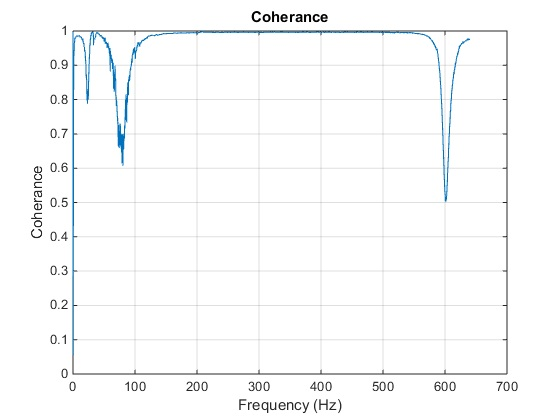
\includegraphics[height=5.50cm]{baseFilt_woWeight_coh.jpg}
		\label{fig:baseFilt_woWeight_coh}
		}
%		\caption{}
		\label{fig:baseCohFigs1}
	\end{figure}
	\begin{figure}[H]
		\centering
		\subfigure[Coherence for base excitation using raw data (FIXED)]
		{
		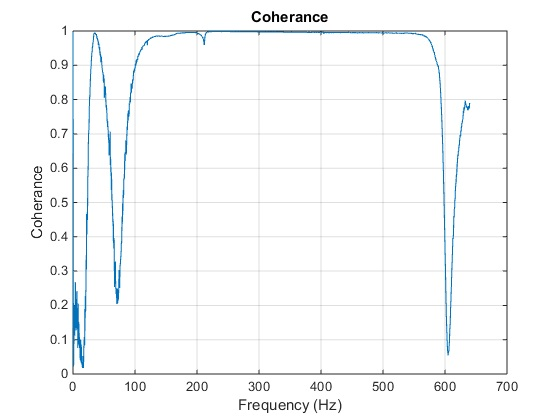
\includegraphics[height=5.50cm]{baseR_wtWeight_coherance.jpg}
		\label{fig:baseR_wtWeight_coherance}
		}
		\quad
		\subfigure[Coherence for base excitation using raw data(LOOSE)]
		{
		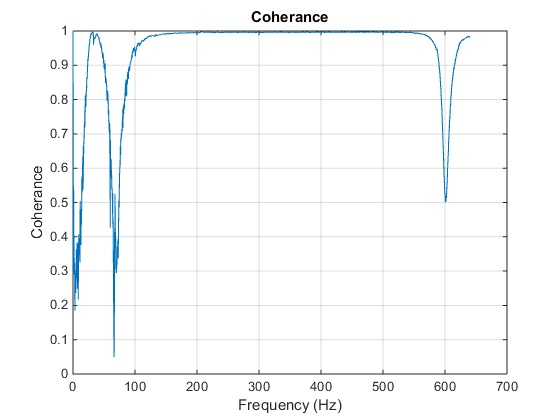
\includegraphics[height=5.50cm]{baseR_woWeight_coherance.jpg}
		\label{fig:baseR_woWeight_coherance}
		}
		\caption{Coherence plots for base excitation. Results shown for FIXED and LOOSE condition.}
		\label{fig:baseCohFigs2}
	\end{figure}
%
In general, Figures~\ref{fig:baseFilt_wtWeight_coh} thru~\ref{fig:baseR_woWeight_coherance} show very good coherence characteristics. Due to noise removal, the filtered coherence plots in Figures~\ref{fig:baseFilt_wtWeight_coh} and~\ref{fig:baseFilt_woWeight_coh} appear smoother in nature especially in the lower frequency range.
\\
\\
Next subsection will show same plots for the LOC4 hammer excitation of the cantilever beam. Figure~\ref{fig:FiltLOC4CSDFigs} shows the CSD results for the filtered and raw data sets.
%
	\begin{figure}[H]
		\centering
		\subfigure[CSD for base excitation using filtered data (FIXED)]
		{
		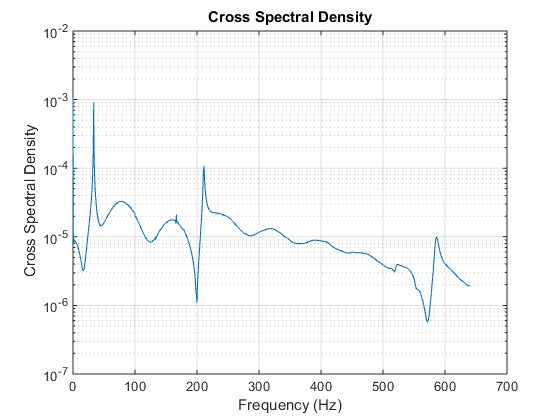
\includegraphics[height=5.50cm]{LOC4Filt_wtWeight_CSD.jpg}
		\label{fig:LOC4Filt_wtWeight_CSD}
		}
		\quad
		\subfigure[CSD for base excitation using filtered data (LOOSE)]
		{
		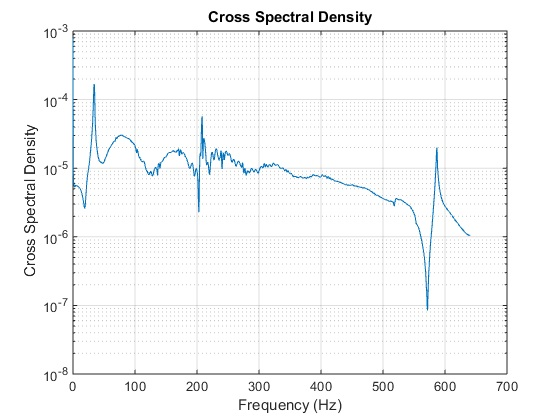
\includegraphics[height=5.50cm]{LOC4Filt_woWeight_CSD.jpg}
		\label{fig:LOC4Filt_woWeight_CSD}
		}
		%\quad
		\subfigure[CSD for base excitation using raw data (FIXED)]
		{
		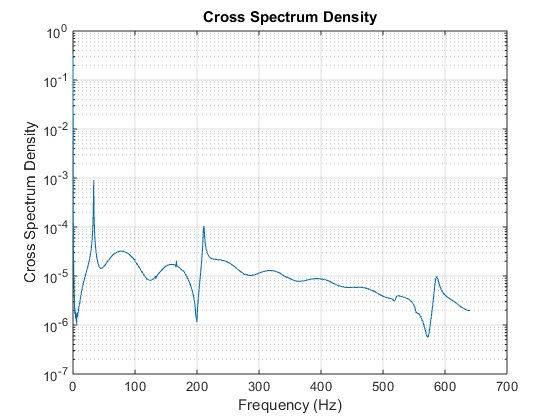
\includegraphics[height=5.50cm]{LOC4R_wtWeight_CSD.jpg}
		\label{fig:LOC4R_wtWeight_CSD}
		}
		%\quad
		\subfigure[CSD for base excitation using raw data(LOOSE)]
		{
		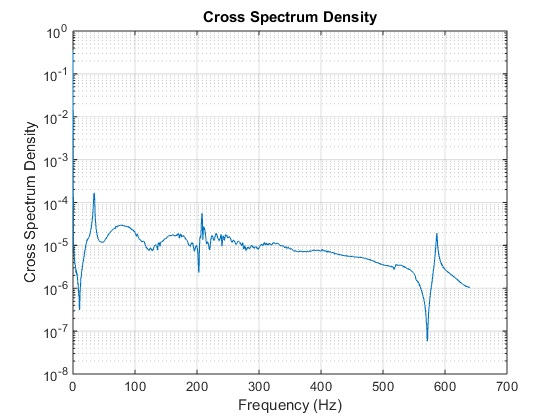
\includegraphics[height=5.50cm]{LOC4R_woWeight_CSD.jpg}
		\label{fig:LOC4R_woWeight_CSD}
		}
		\caption{CSD plots for LOC4 excitation. Results shown for FIXED and LOOSE condition.}
		\label{fig:FiltLOC4CSDFigs}
	\end{figure}
%
Evaluating Figures~\ref{fig:LOC4Filt_wtWeight_CSD} thru~\ref{fig:LOC4R_woWeight_CSD} shows no significant differences except for the early part of the graphs. For the LOOSE condition, Figures~\ref{fig:LOC4Filt_woWeight_CSD} and~\ref{fig:LOC4R_woWeight_CSD} show approximately same levels of noise at the pole located at 200 Hz. This is to be expected since the filter was not applied in this frequency range. Main reason for the noise in this region is due to high noise floor and low pole amplitude, which can be attributed to the unstable fixture.
\\
\\
Figures~\ref{fig:LOC4Filt_wtWeight_H1_H2} thru~\ref{fig:LOC4R_woWeight_H1_H2} show H1 and H2 estimates for the LOOSE condition. Except for the early portion of the plots, Figures~\ref{fig:LOC4Filt_wtWeight_H1_H2} and~\ref{fig:LOC4R_wtWeight_H1_H2} show similar responses for filtered and raw data. Additionally, near pole/zero cancellation at 200 Hz is clearly visible for both cases. In similar fashion Figures~\ref{fig:LOC4Filt_woWeight_H1_H2} and~\ref{fig:LOC4R_woWeight_H1_H2} are almost identical. Both filtered and raw data sets fail to account for the zero at the 200 Hz location. This should not be a surprise since the filter did not act in this frequency range.
%
	\begin{figure}[H]
		\centering
		\subfigure[H1 and H2 for LOC4 excitation using filtered data (FIXED)]
		{
		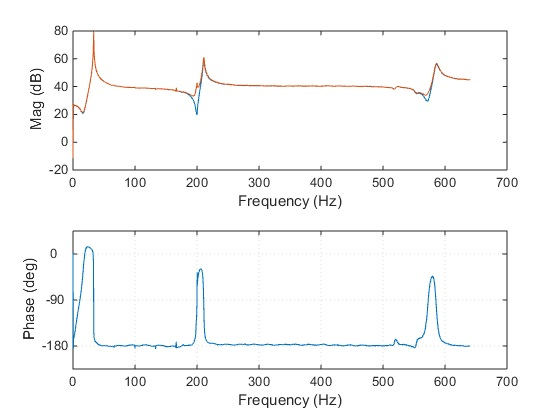
\includegraphics[height=5.50cm]{LOC4Filt_wtWeight_H1_H2.jpg}
		\label{fig:LOC4Filt_wtWeight_H1_H2}
		}
		\quad
		\subfigure[H1 and H2 for LOC4 excitation using filtered data (LOOSE)]
		{
		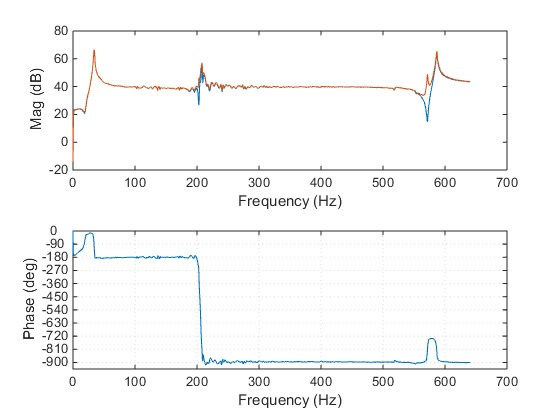
\includegraphics[height=5.50cm]{LOC4Filt_woWeight_H1_H2.jpg}
		\label{fig:LOC4Filt_woWeight_H1_H2}
		}
		%\quad
		\subfigure[H1 and H2 for LOC4 excitation using raw data (FIXED)]
		{
		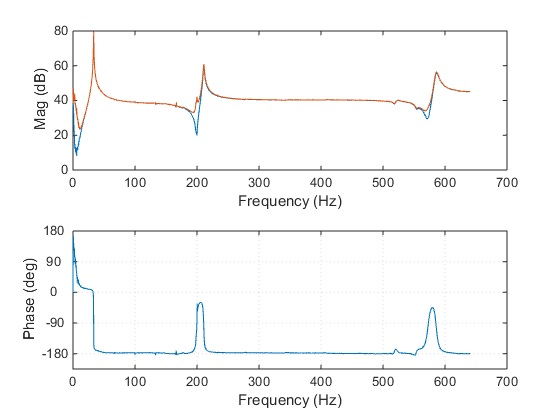
\includegraphics[height=5.50cm]{LOC4R_wtWeight_H1_H2.jpg}
		\label{fig:LOC4R_wtWeight_H1_H2}
		}
		%\quad
		\subfigure[H1 and H2 for LOC4 excitation using raw data(LOOSE)]
		{
		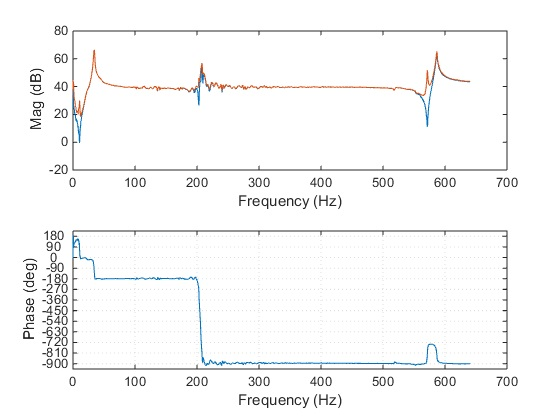
\includegraphics[height=5.50cm]{LOC4R_woWeight_H1_H2.jpg}
		\label{fig:LOC4R_woWeight_H1_H2}
		}
		\caption{H1 and H2 plots for LOC4 excitation. Results shown for FIXED and LOOSE condition.}
		\label{fig:FiltLOC4H1H2Figs}
	\end{figure}
%
Figures~\ref{fig:LOC4Filt_wtWeight_coh} thru~\ref{fig:LOC4R_woWeight_coherance} shows the coherence plots for the LOOSE condition. Coherence plots are similar to the base excitation results. In general the coherence is well defined across the entire frequency range. Filtered plots in Figures~\ref{fig:LOC4Filt_wtWeight_coh} and~\ref{fig:LOC4Filt_woWeight_coh} have a smoother tendency in the early frequency range, which again should be expected.
%
	\begin{figure}[H]
		\centering
		\subfigure[Coherence for LOC4 excitation using filtered data (FIXED)]
		{
		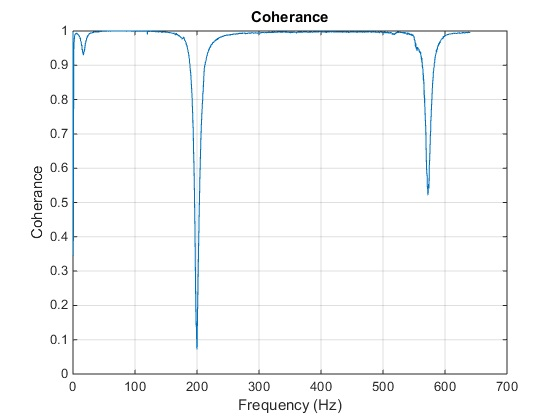
\includegraphics[height=5.50cm]{LOC4Filt_wtWeight_coh.jpg}
		\label{fig:LOC4Filt_wtWeight_coh}
		}
		\quad
		\subfigure[Coherence for LOC4 excitation using filtered data (LOOSE)]
		{
		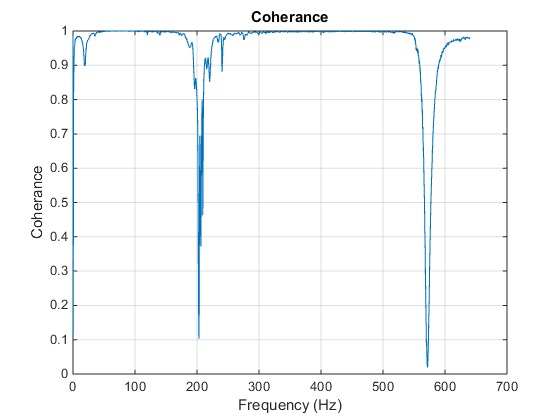
\includegraphics[height=5.50cm]{LOC4Filt_woWeight_coh.jpg}
		\label{fig:LOC4Filt_woWeight_coh}
		}
%		\caption{}
%		\label{fig:baseCohFigs1}
%	\end{figure}
%	\begin{figure}[H]
%		\centering
		\subfigure[Coherence for LOC4 excitation using raw data (FIXED)]
		{
		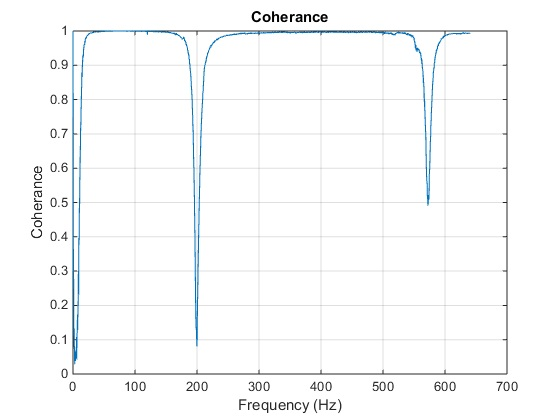
\includegraphics[height=5.50cm]{LOC4R_wtWeight_coherance.jpg}
		\label{fig:LOC4R_wtWeight_coherance}
		}
%		\quad
		\subfigure[Coherence for LOC4 excitation using raw data(LOOSE)]
		{
		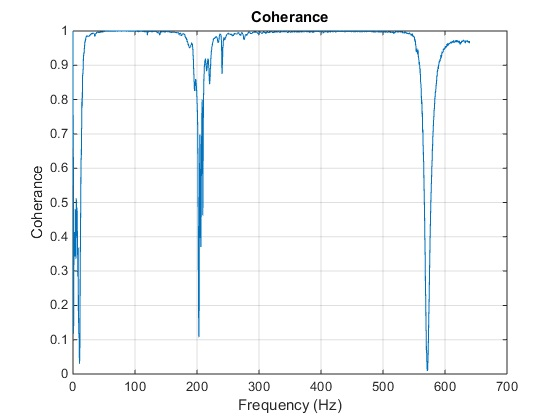
\includegraphics[height=5.50cm]{LOC4R_woWeight_coherance.jpg}
		\label{fig:LOC4R_woWeight_coherance}
		}
		\caption{Coherence plots for LOC4 excitation. Results shown for FIXED and LOOSE condition.}
		\label{fig:LOC4CohFigs2}
	\end{figure}
%
%
\section*{Summary}
A high-pass filter was constructed using Matlab signal processing toolbox. The main intent of the filter was to remove the vertical shift and low frequency drift from the input and output time histories. Applying the filter to the hammer input signal did not produce acceptable results. Therefore, decision was made use raw input signals. A different filtering strategy needs to be developed for the input signals but was not pursued in this report. Applying the filter to the raw beam output time histories did produce agreeable results. The goal of removing the low frequency noise was achieved without adversely affecting the beam response.
\\
\\
Beam time histories were obtained from an earlier experiment, which studied the effect of fixture stability on experimental results. Data sets from this experiment were identified as FIXED and LOOSE. For both of the experimental configurations the beam was excited at two locations. First excitation was performed at the base of the beam while the second was carried out near the end of the beam at location four. These input locations were dubbed 'base' and 'LOC4'.
\\
\\
Filtering procedure was carried out for all the cases mentioned in the above paragraph. After the filtering process, the data contained a horizontal shift, which was removed manually. All the beam output time histories were filtered using same filter parameters. This was done in order to reduce any potential variation due to parameter changes between different data sets.
\\
\\
For FIXED and LOOSE data sets CSD, FRF, and coherence plots were created for the filtered data and compared to raw data calculations. Noise removal is clearly evident in the low frequency range of the aforementioned plots. Estimations of H2 transfer function for the base input data sets possessed an artificial peak, which was responsible for a negative phase shift in Figure~\ref{fig:baseFilt_wtWeight_H1_H2}. It is not clear why this peak is showing up or why filtering process makes it more prominent. Further evaluation is needed to determine root cause. Since filtering only acts in the low frequency range the transfer function estimates and corresponding phase diagrams in Figures~\ref{fig:baseFilt_woWeight_H1_H2} and~\ref{fig:baseR_woWeight_H1_H2} match closely. Both of these figures missed the zero at the 75 Hz location due to the LOOSE condition of the fixture. Coherence plots for base excitation in Figures~\ref{fig:baseFilt_wtWeight_coh} thru~\ref{fig:baseR_woWeight_coherance} show similar behavior except for the beginning of the plot where filtered signals show less noise. For LOC4 excitation, the estimated transfer functions in Figures~\ref{fig:LOC4Filt_wtWeight_H1_H2} and~\ref{fig:LOC4R_wtWeight_H1_H2} show the near pole/zero cancellation. Conversely, for Figures~\ref{fig:LOC4Filt_woWeight_H1_H2} and~\ref{fig:LOC4R_woWeight_H1_H2}, zero at the 200 Hz location is missed due to the fixture instability. Finally, the coherence plots in Figures~\ref{fig:LOC4Filt_wtWeight_coh} thru~\ref{fig:LOC4R_woWeight_coherance} for LOC4 excitation show similar trends. As was the case for base excitation, filtered signals appear smoother due to the filtering operation. 
\\
\\ 
In conclusion, filtering of the output signals did smooth the response by removing low frequency noise. However, no amount of filtering can overcome poor experimental set-up procedures, which can be seen in Figures~\ref{fig:baseFilt_woWeight_H1_H2} and~\ref{fig:LOC4Filt_woWeight_H1_H2}. Therefore, it is critical to take great care during the actual experimental set-up to ensure signal errors are reduced before the data is manipulated in any way.
%
%
%
%
\end{document}